%% Based on a TeXnicCenter-Template by Gyorgy SZEIDL.
%%%%%%%%%%%%%%%%%%%%%%%%%%%%%%%%%%%%%%%%%%%%%%%%%%%%%%%%%%%%%
%
%------------------------------------------------------------
%
\documentclass[a4paper,12pt,reqno]{article}
%----------------------------------------------------------
\usepackage{amsfonts}
\usepackage{graphicx}
\usepackage{geometry}
\usepackage{color}
\usepackage{amssymb,amsmath}
\usepackage{polski}
\usepackage[T1]{fontenc}
\usepackage[utf8]{inputenc}
\usepackage{caption}
\geometry{margin=1.1in}
\usepackage{wrapfig}
\usepackage{lipsum}  
\usepackage{listings}
\usepackage[toc,page]{appendix}
\usepackage{url}
\usepackage{indentfirst} % pierwszy akapit zawsze z wcięciem
\usepackage{subcaption}	% kilka zdjęc w jednej lini
\definecolor{codegreen}{rgb}{0.5, 0.09, 0.09}
\definecolor{codegray}{rgb}{0.5,0.5,0.5}
\definecolor{codepurple}{rgb}{0.58,0,0.82}
\definecolor{backcolour}{rgb}{0.94,0.94,0.94}
\definecolor{gray}{rgb}{0,0.6,0}

\lstdefinestyle{mystyle}{
    backgroundcolor=\color{backcolour},  
    commentstyle=\color{codegreen},
    keywordstyle=\color{blue},
    numberstyle=\tiny\color{codegray},
    stringstyle=\color{codepurple},
		basicstyle=\footnotesize\fontfamily{cmtt}\selectfont,
    breakatwhitespace=false,         
    breaklines=true,
    captionpos=b,
		language=C++,
    keepspaces=true,                 
    numbers=left,                    
    numbersep=5pt,                  
    showspaces=false,                
    showstringspaces=false,
    showtabs=false,                  
    tabsize=2
}
 
\lstset{style=mystyle}
\lstset{literate=%
    *{0}{{{\color{gray}0}}}1
    {1}{{{\color{gray}1}}}1
    {2}{{{\color{gray}2}}}1
    {3}{{{\color{gray}3}}}1
    {4}{{{\color{gray}4}}}1
    {5}{{{\color{gray}5}}}1
    {6}{{{\color{gray}6}}}1
    {7}{{{\color{gray}7}}}1
    {8}{{{\color{gray}8}}}1
    {9}{{{\color{gray}9}}}1
}
%------------------------------------------------------------
\begin{document}

%\begin{figure}[h]
%	\centering
%		
\includegraphics[width=0.40\textwidth]{logo.pdf}
%\end{figure}


\begin{center}

\thispagestyle{empty}

%UNIWERSYTET WROCŁAWSKI\\
\Large 
Uniwersytet Wrocławski\\
Wydział Fizyki i Astronomii\\
\vspace{0.8cm}
\vspace{1.8cm}

\Large Marcin Pietrzak \\
\vspace{3.2cm}
\Large Galeria modeli komputerowych \\
\vspace{1.5cm}
Computer models gallery
\end{center}
\vspace{3.7cm}
\begin{flushright}

\large{ Praca inżynierska na kierunku \\Informatyka Stosowana i Systemy Pomiarowe \\}
\vspace{0.5cm}
\large{ Opiekun \\ dr hab. Maciej Matyka, prof. UWr}
\end{flushright}
\vspace{2.2cm}

\begin{center}
\large Wrocław, \today
\end{center}

\newpage

\tableofcontents

\newpage

\begin{flushleft}
\Large \textbf{Streszczenie}
\end{flushleft}
\vspace{1cm}


 Lorem ipsum dolor sit amet, consectetur adipiscing elit, sed do eiusmod tempor incididunt ut labore et dolore magna aliqua. Ut enim ad minim veniam, quis nostrud exercitation ullamco laboris nisi ut aliquip ex ea commodo consequat. Duis aute irure dolor in reprehenderit in voluptate velit esse cillum dolore eu fugiat nulla pariatur. Excepteur sint occaecat cupidatat non proident, sunt in culpa qui officia deserunt mollit anim id est laborum.

\newpage
\begin{flushleft}
\Large \textbf{Abstract}
\end{flushleft}
\vspace{1cm}


Lorem ipsum dolor sit amet, consectetur adipiscing elit, sed do eiusmod tempor incididunt ut labore et dolore magna aliqua. Ut enim ad minim veniam, quis nostrud exercitation ullamco laboris nisi ut aliquip ex ea commodo consequat. Duis aute irure dolor in reprehenderit in voluptate velit esse cillum dolore eu fugiat nulla pariatur.

\newpage

\section{Wstęp}

\subsection{Wprowadzenie}

W pewnych aspektach życia człowiek zastanawia się nad paroma rzeczami, czy nie
jesteśmy sami w kosmosie, kiedy nastąpi koniec, czy VR umarł, czy nie jesteśmy
programem komputerowym. Pewnie nie poznamy odpowiedzi na te wszystkie
pytania, jeszcze przez jakiś czas, ale dzisiaj jedno jest pewne. VR na pewno jeszcze
nie umarł i ma się całkiem dobrze. W ciągu ostatnich kilku lat rynek gogli VR zaczął
na nowo się rozwijać, powstało wiele gogli, a do najpopularniejszych z nich należą:
PlayStation VR, Valve Index, HTC Vive Pro \cite{popularnosc_gogli}. Każde z tych gogli ma jednak wady, a
do najważniejszych należy to, że nie są to sprzęty typu plug and play. Trzeba się nie
tylko męczyć z splątaniną przewodów, ale także gogle jak np. Valve Index wymagają
stacji, dzięki którym gogle wiedzą gdzie znajdujesz się przestrzeni 3D. Kolejnym
problemem jest oczywiście cena samego sprzętu który w większości przekracza
ponad 3000 PLN za całość. Jedynie co się z tego zestawu różni to PlayStation VR,
same są jednak przestarzałe, a Sony zapowiedziało ich następcę którego premiera
nastąpi pod koniec 2022 roku \cite{PlayStation_VR2}. Same gogle Sony nie rozwiązały dla mnie
największego problemu, czyli obowiązek podłączenia przewodem, jednakże ten
problem na szczęście rozwiązała już inna firma, mowa oczywiście o Oculus znaną
obecnie jako Reality Labs, jedna z podfirm Facebooka obecnie znana jako Meta. Firma zaczęła
sprzedawać w 2019 gogle Oculus Quest, które były rewolucyjne z jednego ważnego
powodu, były autonomiczne, tzn. nie potrzebowały komputera do obsługi gogli,
ponieważ wystarczą do tego same gogle z kontrolerami ruchowymi. Same gogle nie
potrzebowały też stacji do określania położenia gogli, gdyż same w sobie mają diody
podczerwone które do tego służą. Oculus Quest okazał się dość rewolucyjnym
sprzętem wartym ok. 2000 pln za wersję podstawową, a rok później Oculus wypuścił
następcę za którego zapłaciliśmy jeszcze mniej czyli ok. 1500 pln w wersji
podstawowej. Nie odbyło się to bez kompromisów takich jak: Brak płynnej zmiany
rozstawu soczewek dla oczu, gorszej jakości pasek na głowę, brak magnetycznego
zabezpieczenia pojemnika na baterię. To nie znaczy oczywiścię, że gogle były
gorszę a do najważniejszych należą: Zwiększona roździelość obrazu dla jednego
oka, zmiana procesora na wydajniejszy, wydłużony czas pracy kontrolerów na jednej
baterii \cite{porownanie_gogli}. 

\begin{figure}[!ht]%
	\centering
	\begin{subfigure}{.5\textwidth}
		\centering
		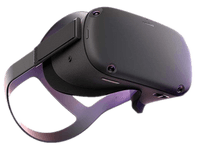
\includegraphics[width=0.8\linewidth]{graphics/oculusquest.png}
		\caption{Oculus Quest 1}	
		\label{ref:subref_a}
	\end{subfigure}%
	\begin{subfigure}{.5\textwidth}
		\centering
		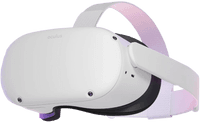
\includegraphics[width=0.8\linewidth]{graphics/oculusquest2.png}
		\caption{Oculus Quest 2}
		\label{ref:subref_b}
	\end{subfigure}%
	

\caption{Gogle VR od Oculusa}
\label{ref:ref}
\end{figure}

Quest 2 wśród gogli VR okazał się dużym sukcesem, w roku 2021
sprzedanych zostało 11,2 miliona sztuk urządzeń z czego 78\% to były Oculus Quest
2 \cite{Sprzedasz_gogli_VR}. Rynek aplikacji też się rozwinął w ciągu ostatnich lat. Na samego Oculusa Questa
w oficjalnym sklepie jest obecnie dostępnych ponad 300 aplikacji, na Steam jest ich
już ponad 2000. Oczywiście wśród nich nie znajdują się same gry, ponieważ gogle
mogą być wykorzystane też np. do zaprezentowania ciała człowieka, być platformą
do rysowania obrazów, lub sprzętem do relaksu czy oglądania filmów. Ja chciałem
spróbować swoich sił w stworzeniu małego projektu, który mógłby być wykorzystany
do pokazywania co ciekawego można robić w komputerze, czyli galerii modelów
komputerowych.

\begin{figure}[!ht]%
\centering
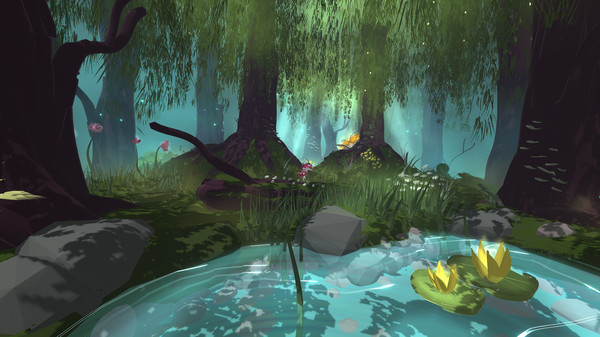
\includegraphics[width=0.8\columnwidth]{graphics/OpenBrush.png}
\caption{OpenBrush
\label{OpenBrush}}%
%
\qquad
\end{figure}  

\subsection{Cel i zakres pracy}

Głównym założeniem jest stworzenie aplikacji VR która przedstawi kilka wybranych
przeze mnie modeli komputerowych w przystępny sposób, łącznie z częścią galerii w
której znajdować się będzie historia danego modelu i ciekawostki z nim związane.
Gogle VR których używałem do testów to Oculus Quest pierwszej generacji,
natomiast aplikację napisałem w Unreal Engine 4, ponieważ mogę w tym silniku
pisać w języku C++, który to najbardziej z języków programowania znam, oraz w
blueprintach czyli Unrealowym wizualnym języku skryptowym, który jest przystępny
dla nowych użytkowników. Silnik posiada pełne wsparcie dla gogli VR czy to wersji
autonomicznej czy wersji PCVR. Sam aplikację pisałem z myślą o PCVR, ponieważ
nie musiałem się aż tak obawiać o ograniczenia które stawia sprzęt w wersji
androidowej np. brak wsparcia dla Unrealowych postprocesów obrazu. Projekt ten
pokazuję, że w dzisiejszych czasach dzięki dostępnym narzędziom typu UE4 i gogle
VR, człowiek jest w stanie stworzyć program w mało wymagający sposób który nie
byłby możliwy do zrealizowania jeszcze 10 lat temu.

\newpage
\section{Warstwa Użytkowa}

\subsection{Wygląd i Obsługa programu}
\subsection{Cześć Galerii Programu}
\subsection{Część pokazowa modeli programu programu}

\section{Warstwa Programistyczna}

\subsection{Język C++}
\subsection{Unreal Engine 4}


\section{Jakie modele się znajdują}

\subsection{Gra w życie}
\subsubsection{Gra w życie - kod}
\subsection{Wahadło Podwójne}
\subsubsection{Wahadło Podwójne - kod}
\subsection{Motyl}
\subsubsection{Motyl - kod}
\subsection{Model Agentowy}
\subsubsection{Model Agentowy - kod}
\subsection{Boids}
\subsubsection{Boids - kod}



\section{Realizacja projektu}

\section{Wnioski}


\newpage

\bibliographystyle{unsrt}
\bibliography{bibliografia}


\end{document}




